\documentclass[11pt,a4paper,landscape]{article}
\usepackage[utf8]{inputenc}
\usepackage[T1]{fontenc}
\usepackage{tikz}
\usepackage{pgfplots}
\pgfplotsset{compat=1.18}
\usepackage{geometry}
\geometry{margin=1in}
\usepackage{xcolor}
\usepackage{amssymb} % Required for \checkmark

% Define aesthetic color palette
\definecolor{primarybg}{HTML}{FFFFFF} % Clean white
\definecolor{boxbg}{HTML}{F8FAFC} % Slate 50
\definecolor{boxbd}{HTML}{CBD5E1} % Slate 300
\definecolor{textmain}{HTML}{1E293B} % Slate 800
\definecolor{textlight}{HTML}{64748B} % Slate 500
\definecolor{accent}{HTML}{2563EB} % Blue 600

\usetikzlibrary{shapes.geometric, arrows.meta, positioning, calc, shadows.blur, fit}

\begin{document}

\pagestyle{empty} % Remove page numbers for clean screenshots

%%%%%%%%%%%%%%%%%%%%%%%%%%%%%%%%%%%%%%%%%%%%%%%%%%%%%%%%%%%%%%%%%%%%%%
% FIGURE 1: RIGOROUS SIGNAL PREPROCESSING PIPELINE (Slide 10)
%%%%%%%%%%%%%%%%%%%%%%%%%%%%%%%%%%%%%%%%%%%%%%%%%%%%%%%%%%%%%%%%%%%%%%
\begin{center}
    \vspace*{2cm}
    \textbf{\Large Figure 1: Rigorous Signal Preprocessing Pipeline} \\
    \vspace{1cm}
    
    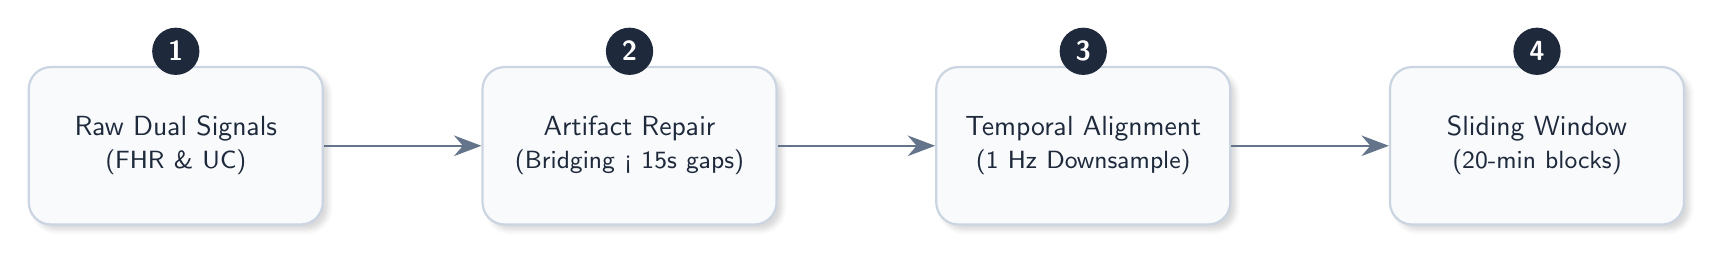
\begin{tikzpicture}[
        node distance=1.5cm and 2cm,
        box/.style={
            rectangle, 
            rounded corners=8pt, 
            draw=boxbd, 
            thick, 
            fill=boxbg, 
            text width=3.5cm, 
            align=center, 
            minimum height=2cm,
            blur shadow={shadow blur steps=5, shadow xshift=2pt, shadow yshift=-2pt, shadow opacity=15},
            font=\sffamily\color{textmain}
        },
        arrow/.style={
            -{Stealth[scale=1.5]}, 
            draw=textlight, 
            thick
        },
        badge/.style={
            circle,
            fill=textmain,
            text=white,
            font=\sffamily\bfseries,
            inner sep=2pt,
            minimum size=6mm
        }
    ]

    % Nodes
    \node[box] (step1) {Raw Dual Signals\\ {\small (FHR \& UC)}};
    \node[box, right=of step1] (step2) {Artifact Repair\\ {\small (Bridging < 15s gaps)}};
    \node[box, right=of step2] (step3) {Temporal Alignment\\ {\small (1 Hz Downsample)}};
    \node[box, right=of step3] (step4) {Sliding Window\\ {\small (20-min blocks)}};

    % Arrows
    \draw[arrow] (step1) -- (step2);
    \draw[arrow] (step2) -- (step3);
    \draw[arrow] (step3) -- (step4);

    % Step Numbers
    \node[badge, shift={(0,1.2)}] at (step1) {1};
    \node[badge, shift={(0,1.2)}] at (step2) {2};
    \node[badge, shift={(0,1.2)}] at (step3) {3};
    \node[badge, shift={(0,1.2)}] at (step4) {4};

    \end{tikzpicture}
\end{center}

\newpage

%%%%%%%%%%%%%%%%%%%%%%%%%%%%%%%%%%%%%%%%%%%%%%%%%%%%%%%%%%%%%%%%%%%%%%
% FIGURE 10: TRI-MODAL STACKING ENSEMBLE ARCHITECTURE (Slide 17)
%%%%%%%%%%%%%%%%%%%%%%%%%%%%%%%%%%%%%%%%%%%%%%%%%%%%%%%%%%%%%%%%%%%%%%
\begin{center}
    \vspace*{3cm}
    \textbf{\Large Figure 10: Tri-Modal Stacking Ensemble Architecture} \\
    \vspace{1cm}
    
    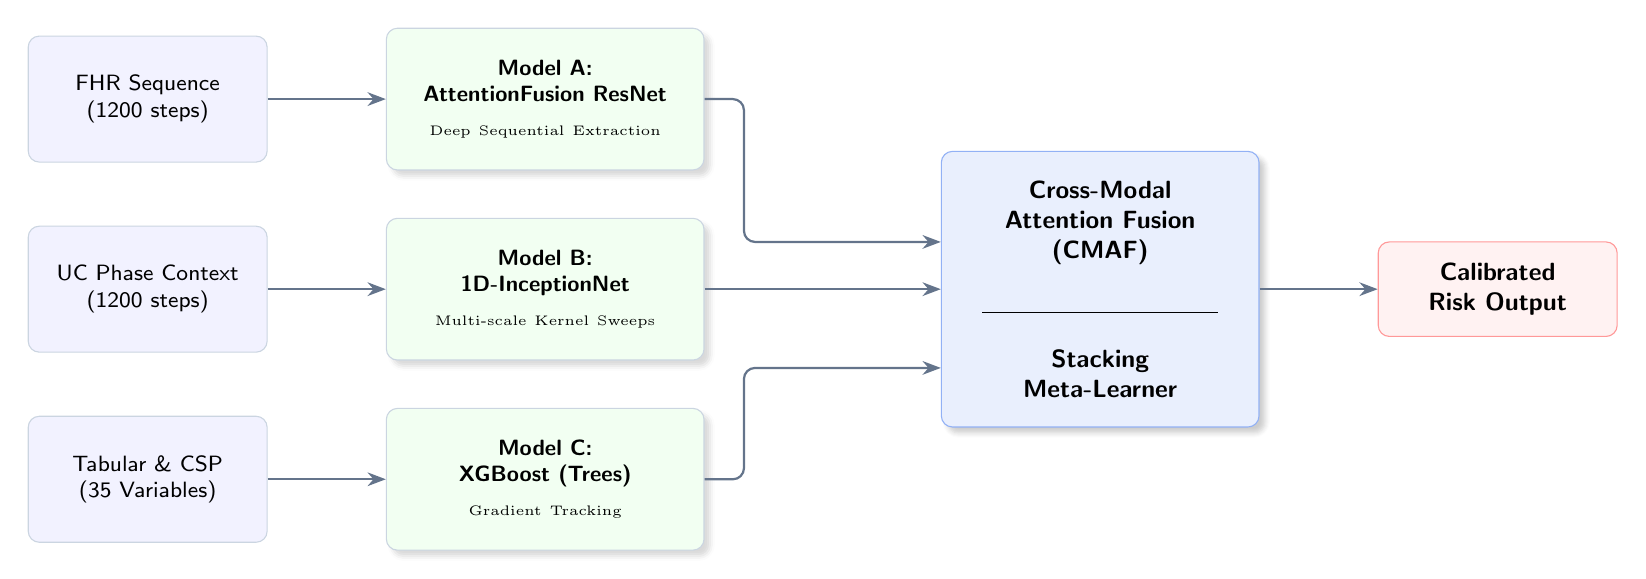
\begin{tikzpicture}[
        node distance=0.8cm and 1.5cm,
        data_node/.style={rectangle, rounded corners, draw=boxbd, fill=blue!5, text width=2.8cm, align=center, minimum height=1.6cm, font=\sffamily\footnotesize},
        model_node/.style={rectangle, rounded corners, draw=boxbd, fill=green!5, text width=3.8cm, align=center, minimum height=1.8cm, font=\sffamily\footnotesize\bfseries, blur shadow={shadow blur steps=3, shadow opacity=15}},
        meta_node/.style={rectangle, rounded corners, draw=accent!50, fill=accent!10, text width=3.8cm, align=center, minimum height=3.5cm, font=\sffamily\small\bfseries, blur shadow={shadow blur steps=5, shadow opacity=20}},
        output_node/.style={rectangle, rounded corners, draw=red!40, fill=red!5, text width=2.8cm, align=center, minimum height=1.2cm, font=\sffamily\small\bfseries},
        arrow/.style={-{Stealth}, draw=textlight, thick}
    ]

    % Data Inputs
    \node[data_node] (fhr) {FHR Sequence\\(1200 steps)};
    \node[data_node, below=of fhr] (uc) {UC Phase Context\\(1200 steps)};
    \node[data_node, below=of uc] (tabular) {Tabular \& CSP\\(35 Variables)};

    % Base Models
    \node[model_node, right=of fhr] (resnet) {Model A:\\AttentionFusion ResNet\\[0.1cm]\normalfont\tiny Deep Sequential Extraction};
    \node[model_node, right=of uc] (inception) {Model B:\\1D-InceptionNet\\[0.1cm]\normalfont\tiny Multi-scale Kernel Sweeps};
    \node[model_node, right=of tabular] (xgboost) {Model C:\\XGBoost (Trees)\\[0.1cm]\normalfont\tiny Gradient Tracking};

    % Meta-Learner (CMAF included here conceptually)
    \node[meta_node, right=of inception, xshift=1.5cm] (fusion) {Cross-Modal\\Attention Fusion\\(CMAF)\\[0.3cm]\rule{3cm}{0.4pt}\\[0.3cm]Stacking\\Meta-Learner};

    % Output
    \node[output_node, right=of fusion] (risk) {Calibrated\\Risk Output};

    % Connections
    \draw[arrow] (fhr) -- (resnet);
    \draw[arrow] (uc) -- (inception);
    \draw[arrow] (tabular) -- (xgboost);

    % Base Models to Fusion
    \draw[arrow, rounded corners=4pt] (resnet.east) -- ++(0.5,0) |- ([yshift=0.6cm]fusion.west);
    \draw[arrow] (inception.east) -- (fusion.west);
    \draw[arrow, rounded corners=4pt] (xgboost.east) -- ++(0.5,0) |- ([yshift=-1.0cm]fusion.west);
    
    \draw[arrow] (fusion) -- (risk);

    \end{tikzpicture}
\end{center}

\newpage

%%%%%%%%%%%%%%%%%%%%%%%%%%%%%%%%%%%%%%%%%%%%%%%%%%%%%%%%%%%%%%%%%%%%%%
% FIGURE 6: AUGMENTATION CHALLENGES (Slide 13 - SMOTE Flaw)
%%%%%%%%%%%%%%%%%%%%%%%%%%%%%%%%%%%%%%%%%%%%%%%%%%%%%%%%%%%%%%%%%%%%%%
\begin{center}
    \vspace*{2cm}
    \textbf{\Large Figure 6: The Biological Failure of SMOTE Mapping} \\
    \vspace{1.5cm}
    
    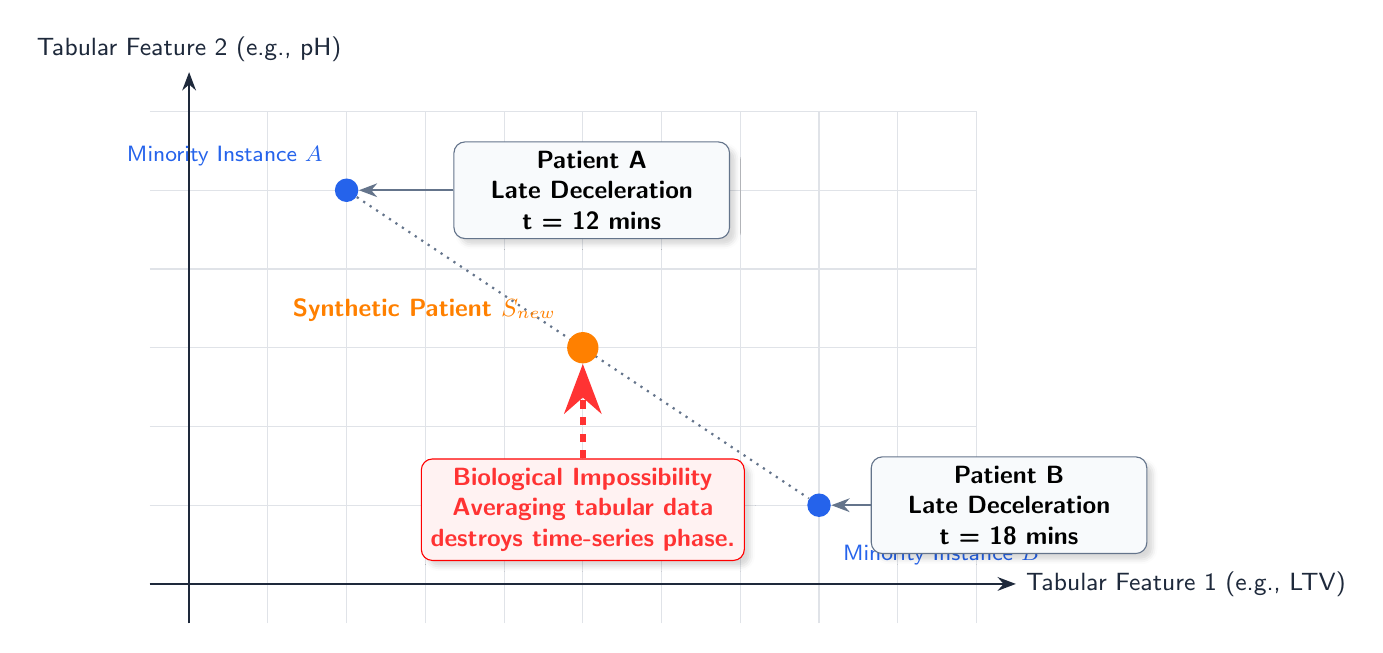
\begin{tikzpicture}[
        font=\sffamily,
        node distance=2cm,
        box/.style={
            rectangle, 
            rounded corners=4pt, 
            draw=textlight, 
            fill=boxbg, 
            align=center, 
            minimum width=3.5cm, 
            minimum height=1cm,
            font=\sffamily\small\bfseries,
            blur shadow={shadow blur steps=3, shadow opacity=15}
        },
        arrow/.style={
            -{Stealth[scale=1.5]}, 
            draw=red!80, 
            line width=2pt,
            dashed
        }
    ]

    % Grid/Background for context
    \draw[step=1cm, textlight!20, thin] (-0.5, -0.5) grid (10, 6);
    \draw[thick, textmain, -Stealth] (-0.5, 0) -- (10.5, 0) node[right] {\small Tabular Feature 1 (e.g., LTV)};
    \draw[thick, textmain, -Stealth] (0, -0.5) -- (0, 6.5) node[above] {\small Tabular Feature 2 (e.g., pH)};

    % Real Data Points
    \node[circle, fill=accent, inner sep=3pt] (p1) at (2, 5) {};
    \node[above left=0.1cm of p1, font=\sffamily\footnotesize, text=accent] {Minority Instance $A$};
    
    \node[circle, fill=accent, inner sep=3pt] (p2) at (8, 1) {};
    \node[below right=0.1cm of p2, yshift=-0.2cm, font=\sffamily\footnotesize, text=accent] {Minority Instance $B$};

    % SMOTE Interpolation Line
    \draw[textlight, thick, dotted] (p1) -- (p2);

    % Synthetic Point
    \node[circle, fill=orange, inner sep=4pt] (s1) at (5, 3) {};
    \node[above left=0.1cm of s1, font=\sffamily\small\bfseries, text=orange] {Synthetic Patient $S_{new}$};

    % Explanatory Boxes
    \node[box, right=1.2cm of p1] (desc1) {Patient A\\Late Deceleration\\t = 12 mins};
    \draw[-{Stealth}, textlight, thick] (desc1) -- (p1);
    
    \node[box, right=0.5cm of p2] (desc2) {Patient B\\Late Deceleration\\t = 18 mins};
    \draw[-{Stealth}, textlight, thick] (desc2) -- (p2);
    
    \node[box, fill=red!5, draw=red, text=red!80, below=1.2cm of s1] (desc_smote) {\textbf{Biological Impossibility}\\Averaging tabular data\\destroys time-series phase.};
    
    \draw[arrow] (desc_smote) -- (s1);

    \end{tikzpicture}
    
    \vspace{0.75cm}
    {\small \sffamily \textit{SMOTE aggressively draws static lines through space without considering time, generating an averaged "Frankenstein" tabular point that corresponds to an impossible physiological waveform constraint.}}
\end{center}

\newpage

%%%%%%%%%%%%%%%%%%%%%%%%%%%%%%%%%%%%%%%%%%%%%%%%%%%%%%%%%%%%%%%%%%%%%%
% FIGURE 7: GENERATIVE METHODOLOGY (Slide 14 - TimeGAN)
%%%%%%%%%%%%%%%%%%%%%%%%%%%%%%%%%%%%%%%%%%%%%%%%%%%%%%%%%%%%%%%%%%%%%%
\begin{center}
    \vspace*{3cm}
    \textbf{\Large Figure 7: WGAN-GP Architecture for Sequential Fidelity} \\
    \vspace{1.5cm}
    
    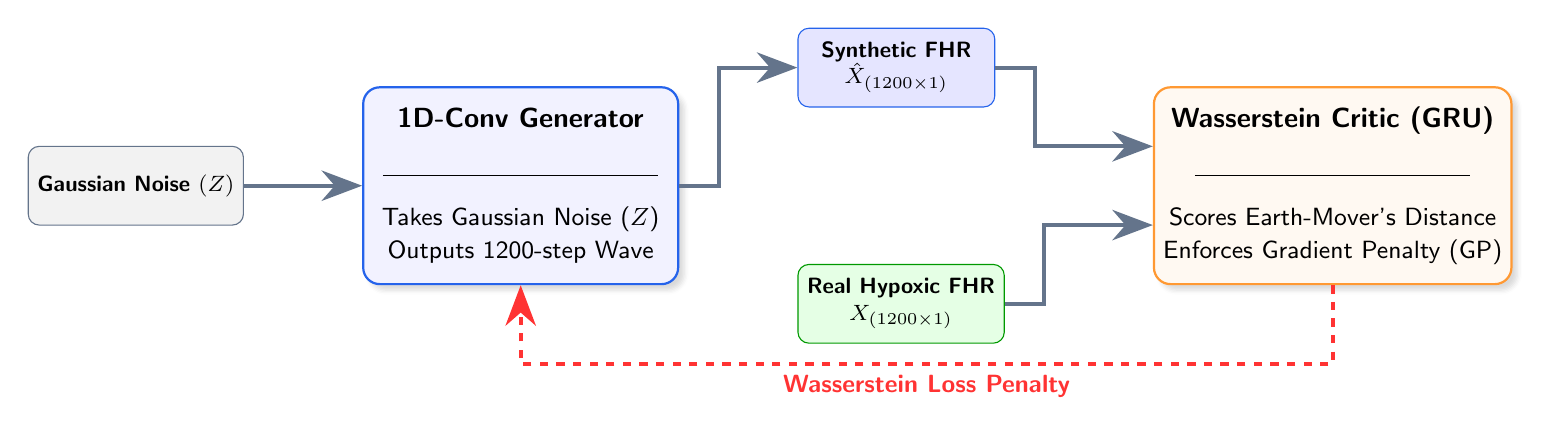
\begin{tikzpicture}[
        node distance=1.5cm and 2cm,
        font=\sffamily,
        net_box/.style={
            rectangle, 
            rounded corners=6pt, 
            draw=boxbd, 
            thick,
            fill=boxbg, 
            align=center, 
            minimum width=4cm, 
            minimum height=2.5cm,
            blur shadow={shadow blur steps=4, shadow opacity=15}
        },
        data_node/.style={
            rectangle, 
            rounded corners=4pt, 
            draw=textlight, 
            fill=white, 
            align=center, 
            minimum width=2.5cm, 
            minimum height=1cm,
            font=\sffamily\footnotesize\bfseries
        },
        loss_node/.style={
            circle, 
            fill=red!10, 
            draw=red!80, 
            thick, 
            align=center, 
            minimum size=1.5cm,
            font=\sffamily\small\bfseries, text=red!80
        },
        arrow/.style={
            -{Stealth[scale=1.5]}, 
            draw=textlight, 
            line width=1.5pt
        }
    ]

    % Generator Branch (Left)
    \node[data_node, fill=gray!10] (noise) {Gaussian Noise $(Z)$};
    \node[net_box, right=1.5cm of noise, fill=blue!5, draw=accent] (generator) {\textbf{1D-Conv Generator} \\[0.2cm] \rule{3.5cm}{0.4pt} \\[0.2cm] \small Takes Gaussian Noise ($Z$) \\ \small Outputs 1200-step Wave};
    \draw[arrow] (noise) -- (generator);

    % Outputs
    \node[data_node, right=1.5cm of generator, yshift=1.5cm, fill=blue!10, draw=accent] (fake) {\textbf{Synthetic FHR}\\$\hat{X}_{(1200\times1)}$};
    \draw[arrow] (generator.east) -- ++(0.5,0) |- (fake.west);

    \node[data_node, right=1.5cm of generator, yshift=-1.5cm, fill=green!10, draw=green!60!black] (real) {\textbf{Real Hypoxic FHR}\\$X_{(1200\times1)}$};

    % Discriminator Branch (Right)
    \node[net_box, fill=orange!5, draw=orange!80, right=2cm of fake, yshift=-1.5cm] (discriminator) {\textbf{Wasserstein Critic (GRU)} \\[0.2cm] \rule{3.5cm}{0.4pt} \\[0.2cm] \small Scores Earth-Mover's Distance \\ \small Enforces Gradient Penalty (GP)};
    
    % Arrows feeding the Critic
    \draw[arrow] (fake.east) -- ++(0.5,0) |- ([yshift=0.5cm]discriminator.west);
    \draw[arrow] (real.east) -- ++(0.5,0) |- ([yshift=-0.5cm]discriminator.west);
    
    % Critic Feedback Loop
    \draw[arrow, red!80, dashed] (discriminator.south) -- ++(0,-1) -| (generator.south) node[pos=0.25, below, text=red!80, font=\sffamily\small\bfseries] {Wasserstein Loss Penalty};

    \end{tikzpicture}
    
    \vspace{0.75cm}
    {\small \sffamily \textit{By replacing SMOTE with a Time-Series Generative Adversarial Network, we force the Generator to natively output 1200-step biological waves that strictly maintain phase alignment with uterine contexts.}}
\end{center}

%%%%%%%%%%%%%%%%%%%%%%%%%%%%%%%%%%%%%%%%%%%%%%%%%%%%%%%%%%%%%%%%%%%%%%
% FIGURE 4: FEATURE ENGINEERING (Slide 11)
%%%%%%%%%%%%%%%%%%%%%%%%%%%%%%%%%%%%%%%%%%%%%%%%%%%%%%%%%%%%%%%%%%%%%%
\begin{center}
    \vspace*{2cm}
    \textbf{\Large Figure 4: Tri-Modal Feature Engineering Hub} \\
    \vspace{1.5cm}
    
    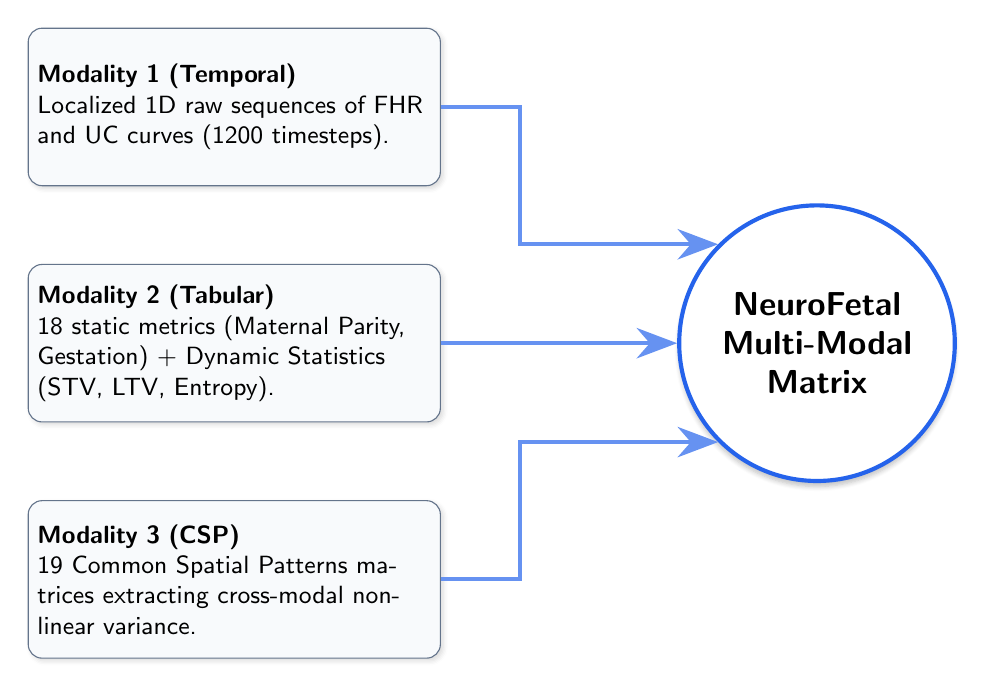
\begin{tikzpicture}[
        node distance=2.5cm and 3cm,
        stream_node/.style={
            rectangle, 
            rounded corners=5pt, 
            draw=textlight, 
            fill=boxbg, 
            text width=5cm, 
            align=left, 
            minimum height=2cm, 
            font=\sffamily\small,
            blur shadow={shadow blur steps=4, shadow xshift=1pt, shadow yshift=-1pt, shadow opacity=15}
        },
        hub_node/.style={
            circle, 
            draw=accent, 
            line width=1.5pt, 
            fill=white, 
            align=center, 
            minimum size=3.5cm, 
            font=\sffamily\bfseries\large,
            blur shadow={shadow blur steps=6, shadow xshift=0pt, shadow yshift=-2pt, shadow opacity=25}
        },
        arrow/.style={
            -{Stealth[scale=1.5]}, 
            draw=accent!70, 
            line width=1.5pt
        }
    ]

    % Central Hub
    \node[hub_node] (hub) {NeuroFetal\\Multi-Modal\\Matrix};

    % Left side streams
    \node[stream_node, left=of hub, yshift=3cm] (mod1) {\textbf{Modality 1 (Temporal)}\\Localized 1D raw sequences of FHR and UC curves (1200 timesteps).};
    \node[stream_node, left=of hub] (mod2) {\textbf{Modality 2 (Tabular)}\\18 static metrics (Maternal Parity, Gestation) + Dynamic Statistics (STV, LTV, Entropy).};
    \node[stream_node, left=of hub, yshift=-3cm] (mod3) {\textbf{Modality 3 (CSP)}\\19 Common Spatial Patterns matrices extracting cross-modal non-linear variance.};

    % Connecting Arrows
    \draw[arrow] (mod1.east) -- ++(1,0) |- (hub.north west);
    \draw[arrow] (mod2.east) -- (hub.west);
    \draw[arrow] (mod3.east) -- ++(1,0) |- (hub.south west);

    \end{tikzpicture}
\end{center}

%%%%%%%%%%%%%%%%%%%%%%%%%%%%%%%%%%%%%%%%%%%%%%%%%%%%%%%%%%%%%%%%%%%%%%
% FIGURE 5: SPECIFIC ALGORITHM (CSP - Slide 12)
%%%%%%%%%%%%%%%%%%%%%%%%%%%%%%%%%%%%%%%%%%%%%%%%%%%%%%%%%%%%%%%%%%%%%%
\begin{center}
    \vspace*{2cm}
    \textbf{\Large Figure 5: Common Spatial Patterns (CSP) Matrix Projection} \\
    \vspace{1.5cm}
    
    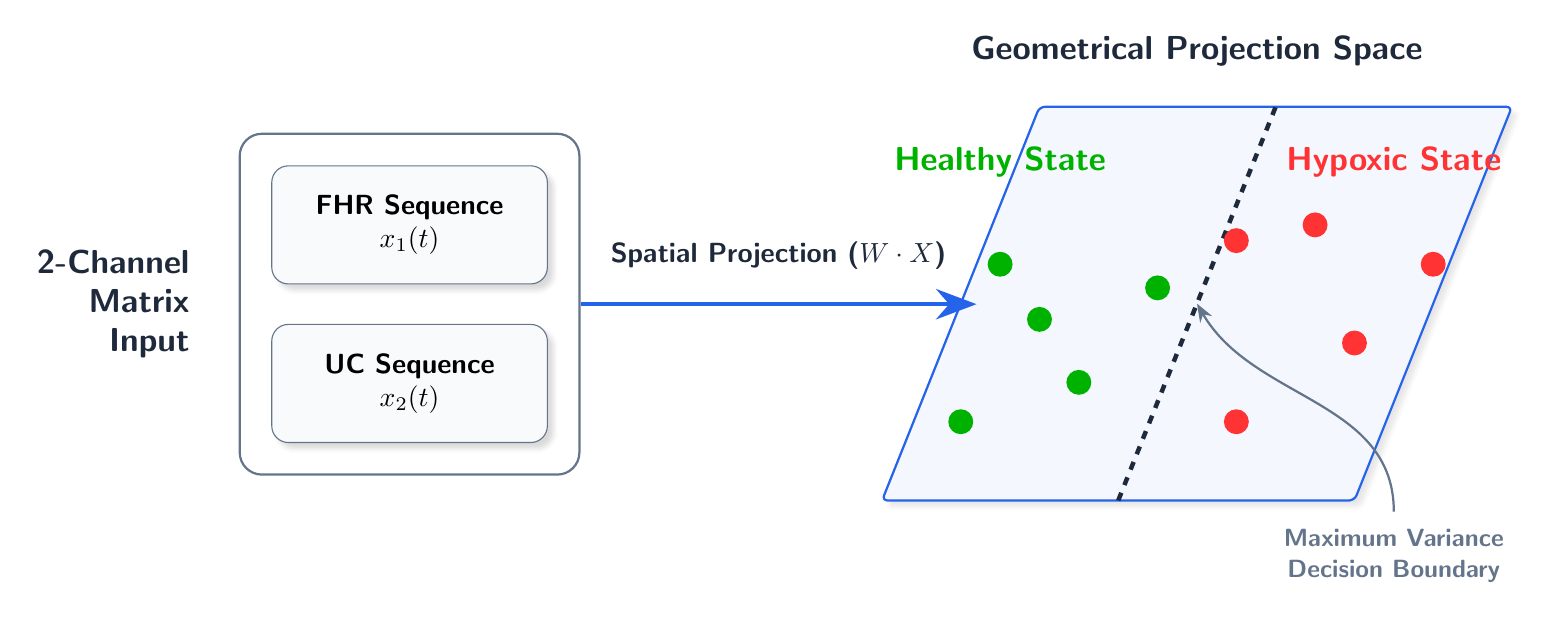
\begin{tikzpicture}[
        node distance=1.5cm and 2cm,
        font=\sffamily,
        wave_box/.style={
            rectangle, 
            rounded corners=6pt, 
            draw=textlight, 
            fill=boxbg, 
            align=center, 
            minimum width=3.5cm, 
            minimum height=1.5cm,
            blur shadow={shadow blur steps=3, shadow opacity=15}
        },
        arrow/.style={
            -{Stealth[scale=1.5]}, 
            draw=accent, 
            line width=1.5pt
        }
    ]

    % Input Waves (Left)
    \node[wave_box] (fhr) {\textbf{FHR Sequence}\\$x_1(t)$};
    \node[wave_box, below=0.5cm of fhr] (uc) {\textbf{UC Sequence}\\$x_2(t)$};
    
    % Grouping Box for Inputs
    \node[
        rectangle, 
        draw=textlight, 
        thick, 
        rounded corners=8pt, 
        fit=(fhr) (uc), 
        inner sep=0.4cm
    ] (input_group) {} node[anchor=east, left=0.5cm of input_group.west, align=right, font=\sffamily\bfseries\large, text=textmain] {2-Channel\\Matrix\\Input};

    % Projection Plane Center
    \coordinate (P_center) at (9, -1);
    
    % The Parallelogram Plane
    \filldraw[fill=accent!5, draw=accent, thick, rounded corners=2pt, blur shadow={shadow blur steps=5, shadow opacity=10}] 
        ($(P_center) + (-3, -2.5)$) -- 
        ($(P_center) + (3, -2.5)$) -- 
        ($(P_center) + (5, 2.5)$) -- 
        ($(P_center) + (-1, 2.5)$) -- cycle;
        
    % Title of the plane (completely clear of dots, centered above plane)
    \node[font=\sffamily\bfseries\large, text=textmain] at ($(P_center) + (1, 3.2)$) {Geometrical Projection Space};

    % Separation Line (Midpoint of bottom to Midpoint of top)
    \coordinate (sep_bottom) at ($(P_center) + (0, -2.5)$);
    \coordinate (sep_top) at ($(P_center) + (2, 2.5)$);
    \draw[textmain, dashed, ultra thick] (sep_bottom) -- (sep_top);
    
    % Decision Boundary Label (Clean, horizontal, pointing to the line from below)
    \node[font=\sffamily\bfseries\small, text=textlight, align=center] (boundary_label) at ($(P_center) + (3.5, -3.2)$) {Maximum Variance\\Decision Boundary};
    \draw[-{Stealth}, textlight, thick] (boundary_label.north) ++(0,0.1) to[out=90, in=300] ($(P_center) + (1, 0)$);

    % Labels for the states
    \node[font=\sffamily\bfseries\large, text=green!70!black] at ($(P_center) + (-1.5, 1.8)$) {Healthy State};
    \node[font=\sffamily\bfseries\large, text=red!80] at ($(P_center) + (3.5, 1.8)$) {Hypoxic State};

    % Scatter points for Healthy (Green) 
    \fill[green!70!black] ($(P_center) + (-1.5, 0.5)$) circle (4.5pt);
    \fill[green!70!black] ($(P_center) + (-0.5, -1.0)$) circle (4.5pt);
    \fill[green!70!black] ($(P_center) + (-2.0, -1.5)$) circle (4.5pt);
    \fill[green!70!black] ($(P_center) + (0.5, 0.2)$) circle (4.5pt); 
    \fill[green!70!black] ($(P_center) + (-1.0, -0.2)$) circle (4.5pt);
    
    % Scatter points for Hypoxic (Red)
    \fill[red!80] ($(P_center) + (1.5, -1.5)$) circle (4.5pt);
    \fill[red!80] ($(P_center) + (3.0, -0.5)$) circle (4.5pt);
    \fill[red!80] ($(P_center) + (2.5, 1.0)$) circle (4.5pt);
    \fill[red!80] ($(P_center) + (4.0, 0.5)$) circle (4.5pt);
    \fill[red!80] ($(P_center) + (1.5, 0.8)$) circle (4.5pt); 
    
    % Arrow from input group to plane (Text gracefully floating above)
    \coordinate (plane_left) at ($(P_center) + (-1.8, 0)$);
    \draw[arrow] (input_group.east) -- (input_group.east -| plane_left) 
        node[midway, above=0.3cm, font=\sffamily\bfseries, text=textmain] {Spatial Projection ($W \cdot X$)};

    \end{tikzpicture}
    
    \vspace{1cm}
    {\small \sffamily \textit{CSP Computationally projects the 2-Channel matrix into a new distinct plane, maximizing the variance disparity strictly between healthy and hypoxic states.}}
\end{center}

%%%%%%%%%%%%%%%%%%%%%%%%%%%%%%%%%%%%%%%%%%%%%%%%%%%%%%%%%%%%%%%%%%%%%%
% FIGURE 8: CORE ARCHITECTURE (Slide 15 - AttentionFusionResNet)
%%%%%%%%%%%%%%%%%%%%%%%%%%%%%%%%%%%%%%%%%%%%%%%%%%%%%%%%%%%%%%%%%%%%%%
\begin{center}
    \vspace*{2cm}
    \textbf{\Large Figure 8: Core Architecture - AttentionFusionResNet} \\
    \vspace{1.5cm}
    
    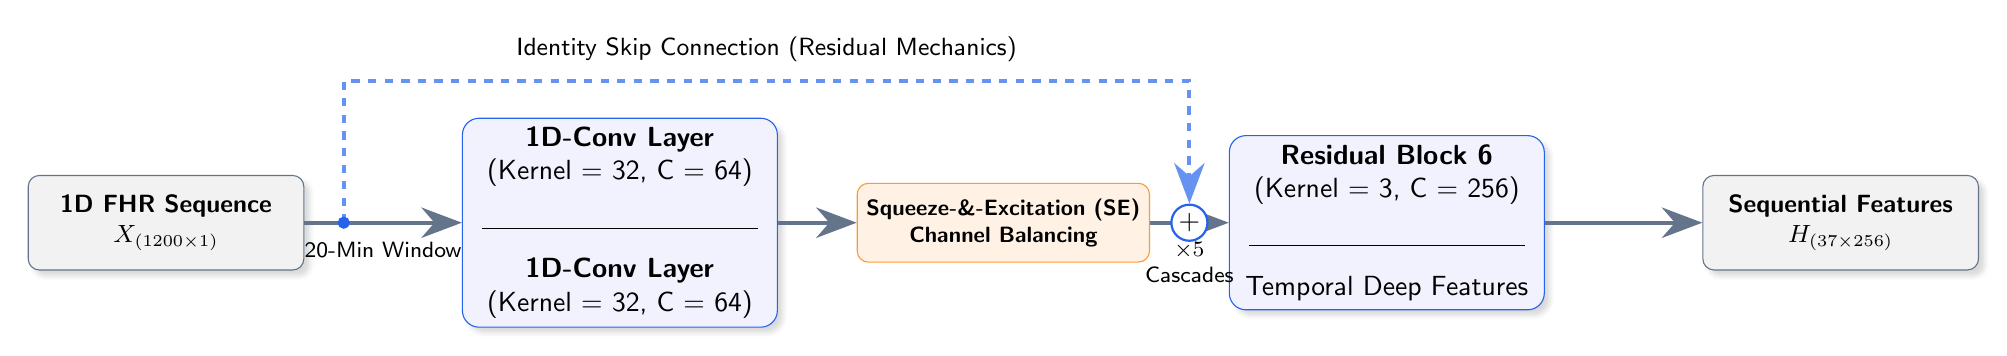
\begin{tikzpicture}[
        node distance=1.5cm and 2cm,
        font=\sffamily,
        data_box/.style={
            rectangle, 
            rounded corners=4pt, 
            draw=textlight, 
            fill=gray!10, 
            align=center, 
            minimum width=3.5cm, 
            minimum height=1.2cm,
            font=\sffamily\small\bfseries,
            blur shadow={shadow blur steps=3, shadow opacity=15}
        },
        res_block/.style={
            rectangle, 
            rounded corners=6pt, 
            draw=accent, 
            fill=blue!5, 
            align=center, 
            minimum width=4cm, 
            minimum height=2cm,
            blur shadow={shadow blur steps=4, shadow xshift=2pt, shadow yshift=-2pt, shadow opacity=15}
        },
        se_block/.style={
            rectangle, 
            rounded corners=4pt, 
            draw=orange!80, 
            fill=orange!10, 
            align=center, 
            minimum width=3.5cm, 
            minimum height=1cm,
            font=\sffamily\footnotesize\bfseries
        },
        arrow/.style={
            -{Stealth[scale=1.5]}, 
            draw=textlight, 
            line width=1.5pt
        },
        skip_arrow/.style={
            -{Stealth[scale=1.5]}, 
            draw=accent!70, 
            line width=1.5pt,
            dashed
        }
    ]

    % Input
    \node[data_box] (input) {1D FHR Sequence \\ $X_{(1200 \times 1)}$};

    % Residual Block 1
    \node[res_block, right=2cm of input] (res1) {\textbf{1D-Conv Layer} \\(Kernel = 32, C = 64) \\[0.2cm] \rule{3.5cm}{0.4pt} \\[0.2cm] \textbf{1D-Conv Layer} \\(Kernel = 32, C = 64)};
    
    % Squeeze-and-Excitation 1
    \node[se_block, right=1cm of res1] (se1) {Squeeze-\&-Excitation (SE)\\Channel Balancing};

    % Residual Block 2 (Represented as cascading)
    \node[res_block, right=1cm of se1] (res2) {\textbf{Residual Block 6} \\(Kernel = 3, C = 256) \\[0.2cm] \rule{3.5cm}{0.4pt} \\[0.2cm] Temporal Deep Features};

    % Output
    \node[data_box, right=2cm of res2] (output) {Sequential Features \\ $H_{(37 \times 256)}$};

    % Main Flow Arrows
    \draw[arrow] (input.east) -- (res1.west) node[midway, below, yshift=-0.1cm, font=\sffamily\footnotesize] {20-Min Window};
    \draw[arrow] (res1.east) -- (se1.west);
    \draw[arrow] (se1.east) -- (res2.west) node[midway, below, yshift=-0.1cm, align=center, font=\sffamily\footnotesize] {$\times 5$\\Cascades};
    \draw[arrow] (res2.east) -- (output.west);

    % Skip Connection Lines
    \node[circle, draw=accent, fill=white, inner sep=1pt, thick] (plus1) at ($(se1.east) + (0.5, 0)$) {$\mathbf{+}$};
    \coordinate (skip_start1) at ($(input.east) + (0.5, 0)$);
    \coordinate (skip_up1) at ($(skip_start1) + (0, 1.8)$);
    
    \draw[skip_arrow] (skip_start1) -- (skip_up1) -| (plus1.north) node[pos=0.25, above, yshift=0.1cm, font=\sffamily\small] {Identity Skip Connection (Residual Mechanics)};
    
    \filldraw[accent] (skip_start1) circle (2pt);

    \end{tikzpicture}
    
    \vspace{1cm}
    {\small \sffamily \textit{The 1D Residual branch utilizes 6 cascading blocks with Squeeze-and-Excitation modules to analyze the raw 20-minute FHR sequence without vanishing gradient degradation.}}
\end{center}

\newpage

%%%%%%%%%%%%%%%%%%%%%%%%%%%%%%%%%%%%%%%%%%%%%%%%%%%%%%%%%%%%%%%%%%%%%%
% FIGURE 9: CROSS-MODAL ATTENTION (Slide 16)
%%%%%%%%%%%%%%%%%%%%%%%%%%%%%%%%%%%%%%%%%%%%%%%%%%%%%%%%%%%%%%%%%%%%%%
\begin{center}
    \vspace*{3cm}
    \textbf{\Large Figure 9: Cross-Modal Attention Fusion (CMAF)} \\
    \vspace{1.5cm}
    
    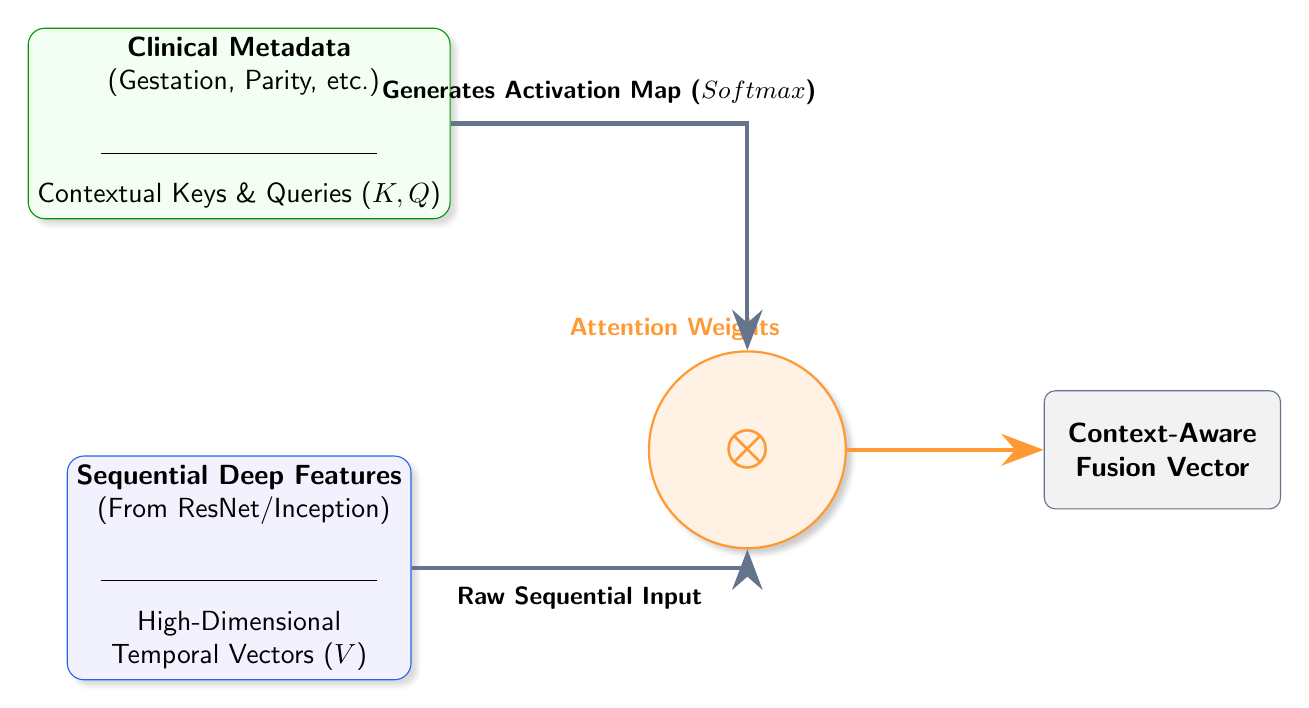
\begin{tikzpicture}[
        node distance=1.5cm and 2cm,
        font=\sffamily,
        seq_node/.style={
            rectangle, 
            rounded corners=6pt, 
            draw=accent, 
            fill=blue!5, 
            align=center, 
            minimum width=4cm, 
            minimum height=2.5cm,
            blur shadow={shadow blur steps=4, shadow opacity=15}
        },
        tab_node/.style={
            rectangle, 
            rounded corners=6pt, 
            draw=green!60!black, 
            fill=green!5, 
            align=center, 
            minimum width=4cm, 
            minimum height=2cm,
            blur shadow={shadow blur steps=4, shadow opacity=15}
        },
        gate_node/.style={
            circle, 
            fill=orange!10, 
            draw=orange!80, 
            thick, 
            align=center, 
            minimum size=2.5cm,
            font=\sffamily\bfseries\Large, text=orange!80,
            blur shadow={shadow blur steps=3, shadow opacity=20}
        },
        arrow/.style={
            -{Stealth[scale=1.5]}, 
            draw=textlight, 
            line width=1.5pt
        }
    ]

    % Sequence Features (Bottom)
    \node[seq_node] (seq) {\textbf{Sequential Deep Features} \\ \vspace{0.1cm} (From ResNet/Inception) \\[0.2cm] \rule{3.5cm}{0.4pt} \\[0.2cm] High-Dimensional\\Temporal Vectors ($V$)};

    % Tabular Features (Top)
    \node[tab_node, above=3cm of seq] (tab) {\textbf{Clinical Metadata} \\ \vspace{0.1cm} (Gestation, Parity, etc.) \\[0.2cm] \rule{3.5cm}{0.4pt} \\[0.2cm] Contextual Keys \& Queries ($K, Q$)};

    % Multiplication Gate (Center)
    \node[gate_node, right=3cm of seq, yshift=1.5cm] (gate) {$\bigotimes$};
    \node[above left=0.1cm of gate, font=\sffamily\small\bfseries, text=orange!80, xshift=1.5cm, yshift=0.3cm] {Attention Weights};

    % Output Vector (Right)
    \node[rectangle, rounded corners=4pt, draw=textlight, fill=gray!10, minimum width=3cm, minimum height=1.5cm, align=center, font=\sffamily\bfseries, right=2.5cm of gate] (output) {Context-Aware\\Fusion Vector};

    % Arrows
    \draw[arrow] (tab.east) -| (gate.north) node[pos=0.25, above, yshift=0.1cm, font=\sffamily\small\bfseries] {Generates Activation Map ($Softmax$)};
    \draw[arrow] (seq.east) -| (gate.south) node[pos=0.25, below, yshift=-0.1cm, font=\sffamily\small\bfseries] {Raw Sequential Input};
    
    \draw[arrow, orange!80, ultra thick] (gate.east) -- (output.west);

    \end{tikzpicture}
    
    \vspace{1.5cm}
    {\small \sffamily \textit{Unlike standard concatenation, CMAF forces Tabular metadata to act as an active mathematical gating key—dynamically amplifying or suppressing temporal sequence weights based on the mother's specific clinical context.}}
\end{center}

\newpage

%%%%%%%%%%%%%%%%%%%%%%%%%%%%%%%%%%%%%%%%%%%%%%%%%%%%%%%%%%%%%%%%%%%%%%
% FIGURE 11: UNCERTAINTY QUANTIFICATION (Slide 18)
%%%%%%%%%%%%%%%%%%%%%%%%%%%%%%%%%%%%%%%%%%%%%%%%%%%%%%%%%%%%%%%%%%%%%%
\begin{center}
    \vspace*{2cm}
    \textbf{\Large Figure 11: Monte Carlo Dropout Variance Analysis} \\
    \vspace{1.5cm}
    
    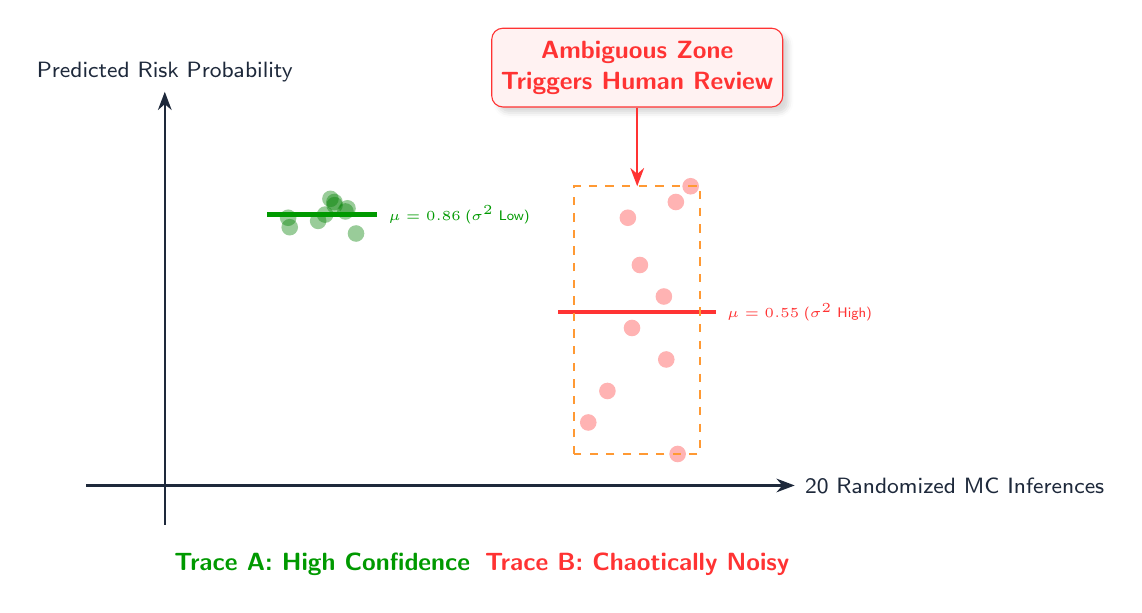
\begin{tikzpicture}[
        font=\sffamily,
        axis/.style={thick, textmain, -Stealth},
        plot_line/.style={draw=accent!40, thick},
        mean_line/.style={draw=accent, ultra thick},
        box/.style={
            rectangle, 
            rounded corners=4pt, 
            draw=red!80, 
            fill=red!5, 
            align=center, 
            minimum width=3cm, 
            minimum height=1cm,
            font=\sffamily\small\bfseries, text=red!80,
            blur shadow={shadow blur steps=3, shadow opacity=15}
        }
    ]

    % Axes
    \draw[axis] (-1, 0) -- (8, 0) node[right, font=\sffamily\footnotesize] {20 Randomized MC Inferences};
    \draw[axis] (0, -0.5) -- (0, 5) node[above, font=\sffamily\footnotesize] {Predicted Risk Probability};

    % High Confidence Example (Left)
    \node[font=\sffamily\small\bfseries, text=green!60!black] at (2, -1) {Trace A: High Confidence};
    \foreach \y in {0.8, 0.85, 0.9, 0.82, 0.88, 0.91, 0.84, 0.87, 0.89, 0.86} {
        \fill[green!50!black, opacity=0.4] (2 + rand*0.5, \y*4) circle (3pt);
    }
    \draw[green!60!black, ultra thick] (1.3, 0.86*4) -- (2.7, 0.86*4) node[right, font=\sffamily\tiny] {$\mu = 0.86$ ($\sigma^2$ Low)};

    % Ambiguous Example (Right)
    \node[font=\sffamily\small\bfseries, text=red!80] at (6, -1) {Trace B: Chaotically Noisy};
    \foreach \y in {0.2, 0.4, 0.9, 0.1, 0.6, 0.85, 0.3, 0.7, 0.5, 0.95} {
        \fill[red!50, opacity=0.6] (6 + rand*0.7, \y*4) circle (3pt);
    }
    \draw[red!80, ultra thick] (5, 0.55*4) -- (7, 0.55*4) node[right, font=\sffamily\tiny] {$\mu = 0.55$ ($\sigma^2$ High)};

    % Variance Range Box
    \draw[draw=orange!80, thick, dashed] (5.2, 0.1*4) rectangle (6.8, 0.95*4);
    
    % Alert Box
    \node[box, above=1cm of {6, 0.95*4}] (alert) {Ambiguous Zone \\ Triggers Human Review};
    \draw[-{Stealth}, red!80, thick] (alert.south) -- (6, 0.95*4);

    \end{tikzpicture}
    
    \vspace{1cm}
    {\small \sffamily \textit{By triggering Monte Carlo Dropout at inference, the model passes the same noisy trace through 20 randomized network states. High spread ($\sigma^2$) prevents dangerous overconfident predictions.}}
\end{center}

\newpage

%%%%%%%%%%%%%%%%%%%%%%%%%%%%%%%%%%%%%%%%%%%%%%%%%%%%%%%%%%%%%%%%%%%%%%
% FIGURE 12: DEPLOYMENT OPTIMIZATION (Slide 20)
%%%%%%%%%%%%%%%%%%%%%%%%%%%%%%%%%%%%%%%%%%%%%%%%%%%%%%%%%%%%%%%%%%%%%%
\begin{center}
    \vspace*{3cm}
    \textbf{\Large Figure 12: TFLite Edge Deployment Pipeline} \\
    \vspace{1.5cm}
    
    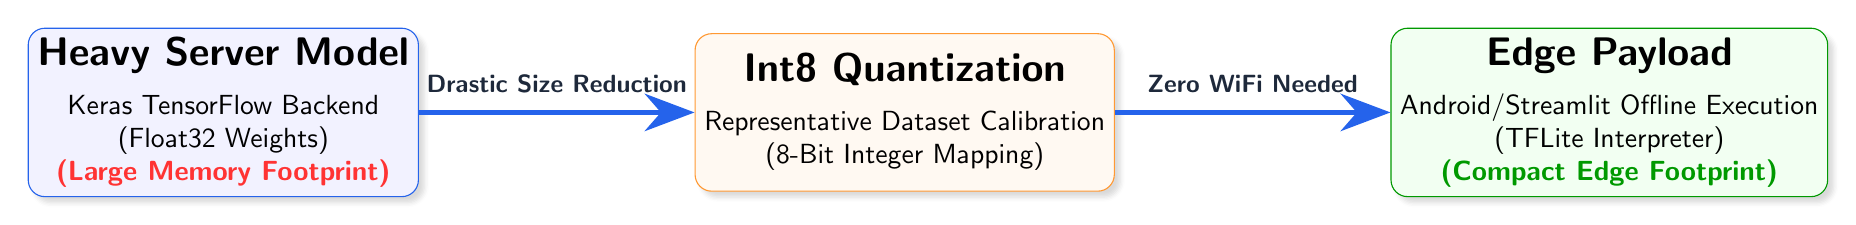
\begin{tikzpicture}[
        node distance=1cm and 3.5cm,
        font=\sffamily,
        stage/.style={
            rectangle, 
            rounded corners=6pt, 
            draw=textlight, 
            fill=boxbg, 
            align=center, 
            minimum width=4.5cm, 
            minimum height=2cm,
            blur shadow={shadow blur steps=4, shadow opacity=15}
        },
        arrow/.style={
            -{Stealth[scale=1.5]}, 
            draw=accent, 
            line width=2pt
        }
    ]

    % Stage 1: GPU Backend
    \node[stage, draw=accent, fill=blue!5] (keras) {\textbf{\Large Heavy Server Model} \\[0.2cm] Keras TensorFlow Backend \\ (Float32 Weights) \\ \textbf{\textcolor{red!80}{(Large Memory Footprint)}}};

    % Stage 2: Quantization
    \node[stage, right=3.5cm of keras, draw=orange!80, fill=orange!5] (quant) {\textbf{\Large Int8 Quantization} \\[0.2cm] Representative Dataset Calibration \\ (8-Bit Integer Mapping)};

    % Stage 3: Edge Payload
    \node[stage, right=3.5cm of quant, draw=green!60!black, fill=green!5] (tflite) {\textbf{\Large Edge Payload} \\[0.2cm] Android/Streamlit Offline Execution \\ (TFLite Interpreter) \\ \textbf{\textcolor{green!60!black}{(Compact Edge Footprint)}}};

    % Arrows
    \draw[arrow] (keras.east) -- (quant.west) node[midway, above, yshift=0.1cm, font=\sffamily\small\bfseries, text=textmain] {Drastic Size Reduction};
    \draw[arrow] (quant.east) -- (tflite.west) node[midway, above, yshift=0.1cm, font=\sffamily\small\bfseries, text=textmain] {Zero WiFi Needed};

    \end{tikzpicture}
    
    \vspace{1.5cm}
    {\small \sffamily \textit{Int8 Quantization crushes massive floating-point architectures into lightweight, rapid 8-bit integers, shrinking the entire NeuroFetal-AI decision support system down to a highly compressed offline file for commodity hardware.}}
\end{center}

\newpage

%%%%%%%%%%%%%%%%%%%%%%%%%%%%%%%%%%%%%%%%%%%%%%%%%%%%%%%%%%%%%%%%%%%%%%
% FIGURE 13: TECHNOLOGY STACK (Slide 21)
%%%%%%%%%%%%%%%%%%%%%%%%%%%%%%%%%%%%%%%%%%%%%%%%%%%%%%%%%%%%%%%%%%%%%%
\begin{center}
    \vspace*{3cm}
    \textbf{\Large Figure 13: NeuroFetal-AI Operational Stack} \\
    \vspace{1.5cm}
    
    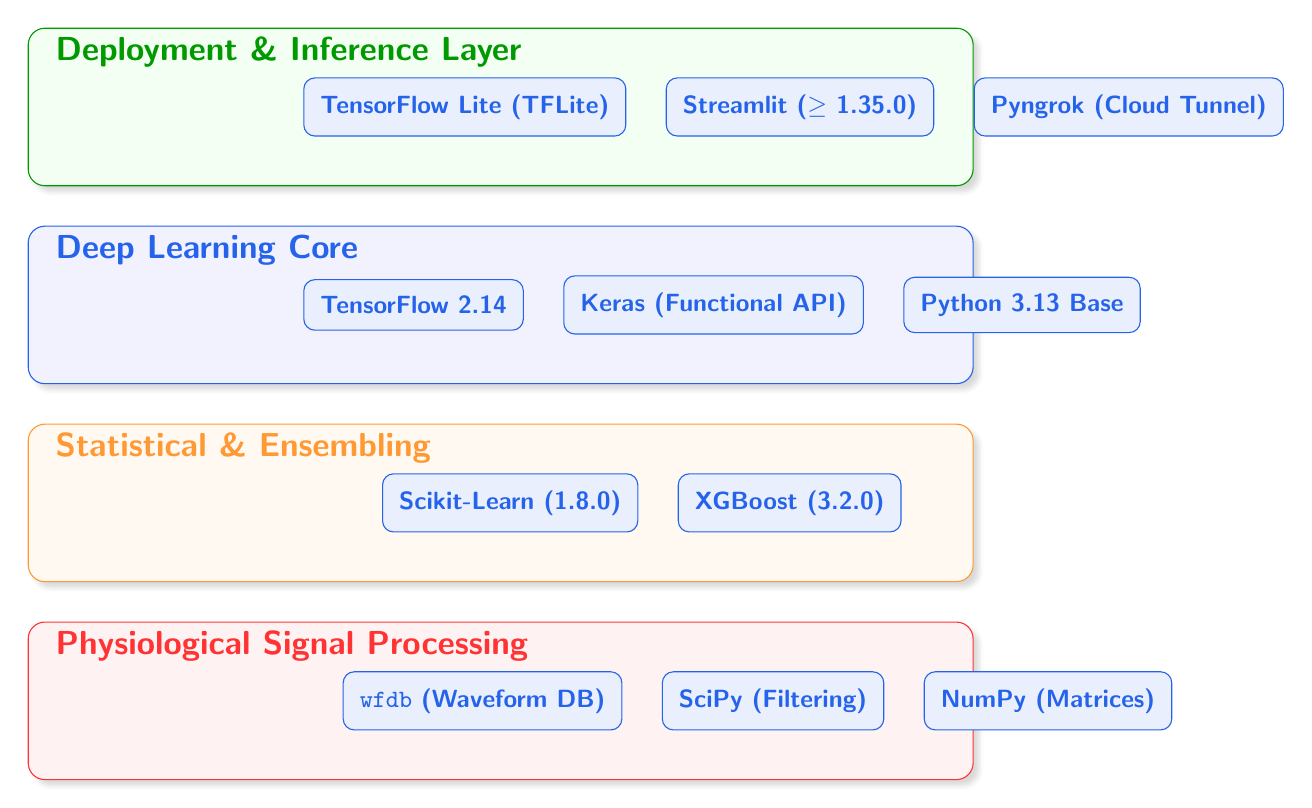
\begin{tikzpicture}[
        node distance=0.5cm and 0.5cm,
        font=\sffamily,
        stack_layer/.style={
            rectangle, 
            rounded corners=6pt, 
            draw=boxbd, 
            fill=white, 
            align=center, 
            minimum width=12cm, 
            minimum height=2cm,
            blur shadow={shadow blur steps=4, shadow opacity=15}
        },
        badge/.style={
            rectangle, 
            rounded corners=4pt, 
            fill=accent!10, 
            text=accent, 
            font=\sffamily\small\bfseries,
            inner sep=6pt,
            draw=accent
        }
    ]

    % Layer 4: Deployment
    \node[stack_layer, fill=green!5, draw=green!60!black] (l4) {};
    \node[anchor=north west, font=\sffamily\bfseries\large, text=green!60!black] at (l4.north west) {\, Deployment \& Inference Layer};
    \node[badge, right=3.5cm of l4.west] (s_tflite) {TensorFlow Lite (TFLite)};
    \node[badge, right=0.5cm of s_tflite] (s_stream) {Streamlit ($\geq$ 1.35.0)};
    \node[badge, right=0.5cm of s_stream] (s_ngrok) {Pyngrok (Cloud Tunnel)};

    % Layer 3: Deep Learning Core
    \node[stack_layer, below=0.5cm of l4, fill=blue!5, draw=accent] (l3) {};
    \node[anchor=north west, font=\sffamily\bfseries\large, text=accent] at (l3.north west) {\, Deep Learning Core};
    \node[badge, right=3.5cm of l3.west] (s_tf) {TensorFlow 2.14};
    \node[badge, right=0.5cm of s_tf] (s_keras) {Keras (Functional API)};
    \node[badge, right=0.5cm of s_keras] (s_py) {Python 3.13 Base};

    % Layer 2: Statistical / Ensembling
    \node[stack_layer, below=0.5cm of l3, fill=orange!5, draw=orange!80] (l2) {};
    \node[anchor=north west, font=\sffamily\bfseries\large, text=orange!80] at (l2.north west) {\, Statistical \& Ensembling};
    \node[badge, right=4.5cm of l2.west] (s_sci) {Scikit-Learn (1.8.0)};
    \node[badge, right=0.5cm of s_sci] (s_xgb) {XGBoost (3.2.0)};

    % Layer 1: Physiological Data Processing
    \node[stack_layer, below=0.5cm of l2, fill=red!5, draw=red!80] (l1) {};
    \node[anchor=north west, font=\sffamily\bfseries\large, text=red!80] at (l1.north west) {\, Physiological Signal Processing};
    \node[badge, right=4cm of l1.west] (s_wfdb) {\texttt{wfdb} (Waveform DB)};
    \node[badge, right=0.5cm of s_wfdb] (s_scipy) {SciPy (Filtering)};
    \node[badge, right=0.5cm of s_scipy] (s_np) {NumPy (Matrices)};

    \end{tikzpicture}
\end{center}

\newpage

%%%%%%%%%%%%%%%%%%%%%%%%%%%%%%%%%%%%%%%%%%%%%%%%%%%%%%%%%%%%%%%%%%%%%%
% FIGURE 14: CONCLUSION & ROADMAP (Slide 22)
%%%%%%%%%%%%%%%%%%%%%%%%%%%%%%%%%%%%%%%%%%%%%%%%%%%%%%%%%%%%%%%%%%%%%%
\begin{center}
    \vspace*{3cm}
    \textbf{\Large Figure 14: Mid-Semester Checkpoint \& Phase 2 Roadmap} \\
    \vspace{2cm}
    
    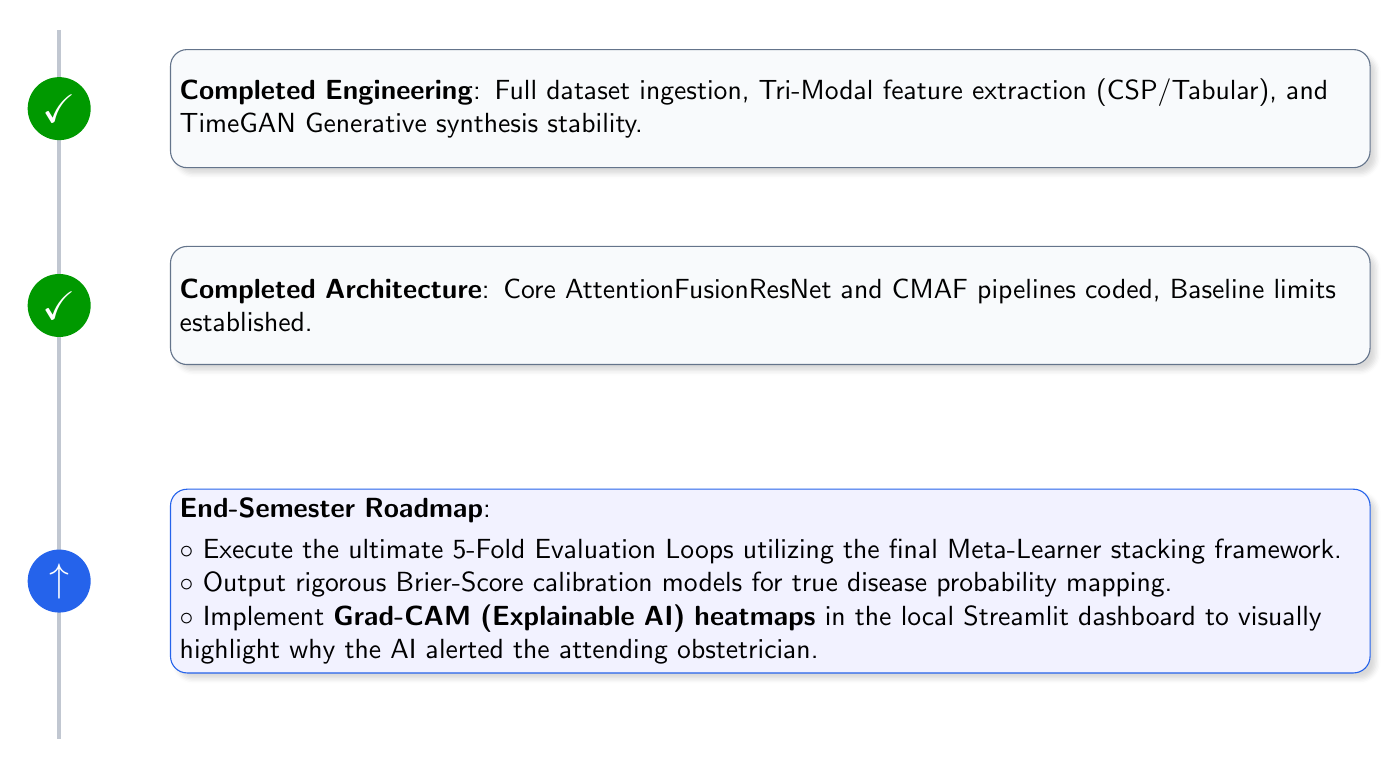
\begin{tikzpicture}[
        node distance=1.5cm,
        font=\sffamily,
        milestone/.style={
            rectangle, 
            rounded corners=6pt, 
            draw=textlight, 
            fill=boxbg, 
            align=left, 
            text width=15cm, 
            minimum height=1.5cm,
            blur shadow={shadow blur steps=4, shadow opacity=15}
        },
        check/.style={
            circle, 
            fill=green!60!black, 
            text=white, 
            font=\sffamily\Large\bfseries, 
            inner sep=2pt, 
            minimum size=0.8cm
        },
        rocket/.style={
            circle, 
            fill=accent, 
            text=white, 
            font=\sffamily\Large\bfseries, 
            inner sep=2pt, 
            minimum size=0.8cm
        }
    ]

    % Connecting Timeline Line
    \draw[ultra thick, textlight!40] (0, 1) -- (0, -8);

    % Milestone 1: Engineering
    \node[check] (c1) at (0, 0) {$\checkmark$};
    \node[milestone, right=1cm of c1] (m1) {\textbf{Completed Engineering}: Full dataset ingestion, Tri-Modal feature extraction (CSP/Tabular), and TimeGAN Generative synthesis stability.};

    % Milestone 2: Architecture
    \node[check] (c2) at (0, -2.5) {$\checkmark$};
    \node[milestone, right=1cm of c2] (m2) {\textbf{Completed Architecture}: Core AttentionFusionResNet and CMAF pipelines coded, Baseline limits established.};

    % Milestone 3: Future Roadmap
    \node[rocket] (c3) at (0, -6) {$\uparrow$};
    \node[milestone, right=1cm of c3, draw=accent, fill=blue!5] (m3) {\textbf{End-Semester Roadmap}: \\[0.1cm]
    $\circ$ Execute the ultimate 5-Fold Evaluation Loops utilizing the final Meta-Learner stacking framework. \\
    $\circ$ Output rigorous Brier-Score calibration models for true disease probability mapping. \\
    $\circ$ Implement \textbf{Grad-CAM (Explainable AI) heatmaps} in the local Streamlit dashboard to visually highlight why the AI alerted the attending obstetrician.};

    \end{tikzpicture}
\end{center}

% =================================================================================
% SLIDE 19: Platt Scaling Calibration Plot
% =================================================================================
\begin{figure}[htbp]
    \centering
    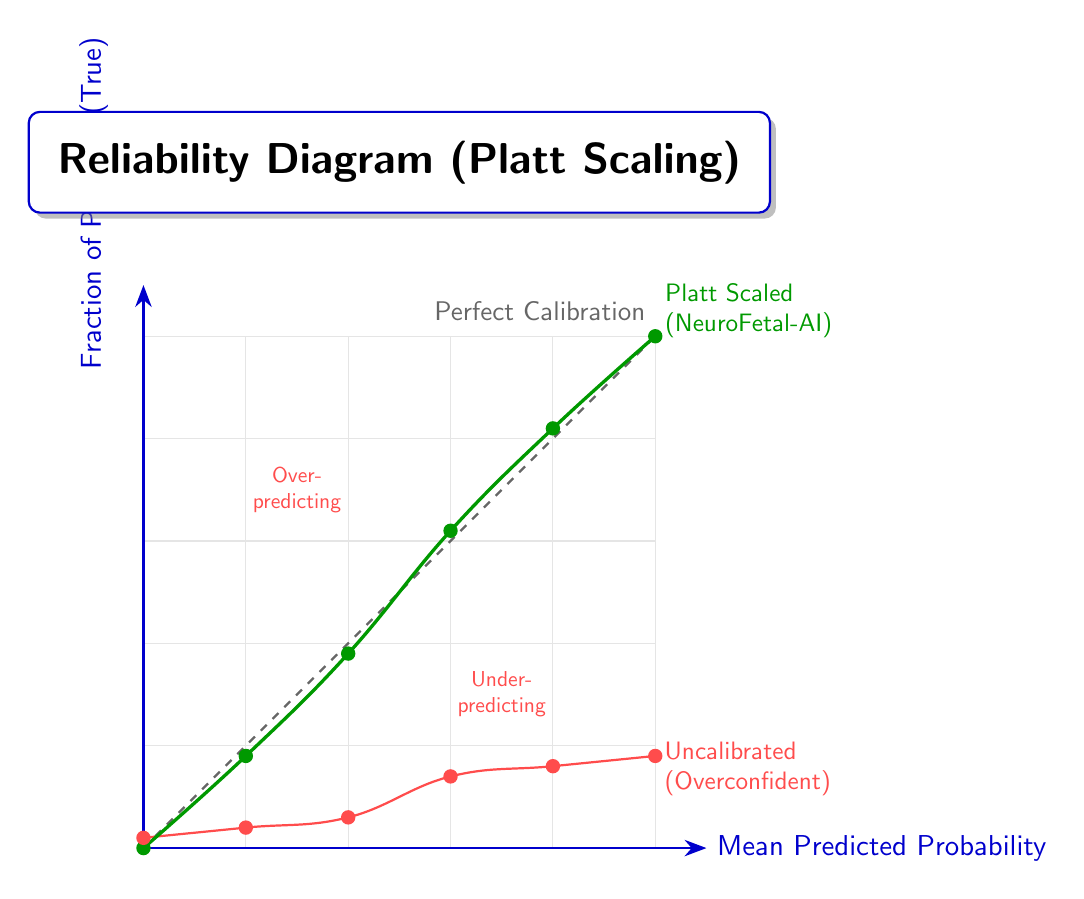
\begin{tikzpicture}[
        font=\sffamily,
        >={Stealth[scale=1.2]},
        scale=1.3, transform shape
    ]
        
        % Background grid and axes
        \draw[step=1cm, gray!20, thin] (0,0) grid (5,5);
        \draw[->, thick, blue!80!black] (0,0) -- (5.5,0) node[right, scale=0.8] {Mean Predicted Probability};
        \draw[->, thick, blue!80!black] (0,0) -- (0,5.5) node[above, rotate=90, scale=0.8, xshift=1cm, yshift=0.3cm] {Fraction of Positives (True)};
        
        % Ideal Perfect Calibration Line (Diagonal)
        \draw[dashed, thick, black!60] (0,0) -- (5,5) node[anchor=south east, sloped, scale=0.75, yshift=2pt] {Perfect Calibration};
        
        % Uncalibrated Model Curve (Sigmoidal distortion)
        \draw[thick, red!70, smooth, tension=0.7] plot coordinates {(0,0.1) (1,0.2) (2,0.3) (3,0.7) (4,0.8) (5,0.9)} 
        node[right, align=left, scale=0.7, yshift=-5pt] {Uncalibrated\\(Overconfident)};
        
        % Calibrated Model Curve (closer to diagonal)
        \draw[very thick, green!60!black, smooth, tension=0.7] plot coordinates {(0,0) (1,0.9) (2,1.9) (3,3.1) (4,4.1) (5,5)} 
        node[right, align=left, scale=0.7, yshift=10pt] {Platt Scaled\\(NeuroFetal-AI)};
        
        % Data points for Calibrated
        \foreach \x/\y in {0/0, 1/0.9, 2/1.9, 3/3.1, 4/4.1, 5/5} {
            \fill[green!60!black] (\x,\y) circle (2pt);
        }
        
        % Data points for Uncalibrated
        \foreach \x/\y in {0/0.1, 1/0.2, 2/0.3, 3/0.7, 4/0.8, 5/0.9} {
            \fill[red!70] (\x,\y) circle (2pt);
        }
        
        % Highlight region (Under-confidence vs Over-confidence)
        \node[red!70, scale=0.6, align=center] at (1.5, 3.5) {Over-\\predicting};
        \node[red!70, scale=0.6, align=center] at (3.5, 1.5) {Under-\\predicting};

        % Title Box
        \node[
            fill=white, 
            draw=blue!80!black, 
            thick, 
            rounded corners, 
            inner sep=8pt,
            drop shadow
        ] at (2.5, 6.7) {\textbf{\large Reliability Diagram (Platt Scaling)}};

    \end{tikzpicture}
    \vspace{0.3cm}
    \caption{Platt Scaling Calibration: Aligning raw model logits perfectly with true disease frequencies via Sigmoid transformations.}
\end{figure}

\end{document}
